\documentclass[acmlarge,manuscript,screen,review]{acmart}

%%% Packages
\usepackage{booktabs}
\usepackage{subcaption}
\usepackage{multirow}
\usepackage{enumitem}

%%% Remove default ACM copyright/conference for manuscript mode
\setcopyright{none}
\settopmatter{printacmref=false, printccs=true, printfolios=true}
\acmJournal{TIST}
\acmYear{2026}

%%% CCS Concepts
\ccsdesc[500]{Computing methodologies~Neural networks}
\ccsdesc[500]{Computer systems organization~Heterogeneous (hybrid) systems}
\ccsdesc[300]{General and reference~Measurement}
\ccsdesc[300]{Computing methodologies~Machine learning}

\keywords{Energy efficiency, generative AI, inference benchmarking, edge computing, scaling laws, hardware selection, sustainable AI}

%%% Title
\title{The Energy Crossover Effect: How Model Architecture Shapes Hardware Efficiency for Generative AI Deployment}

%%% Author
\author{Yongjun Kim}
\email{yjkim@ajou.ac.kr}
\orcid{0000-0003-4234-4883}
\affiliation{%
  \institution{Department of Software, Ajou University}
  \city{Suwon}
  \country{South Korea}
}

\begin{document}

\begin{abstract}
Generative AI systems now serve billions of daily queries spanning text, image, video, and music, yet practitioners lack empirical guidance on which hardware platform minimizes energy for a given workload.
We benchmark three hardware tiers---edge SoC (Apple M4 Pro, 22\,W TDP), mainstream GPU (NVIDIA A100, 400\,W), and high-end GPU (NVIDIA H100, 700\,W)---across 4,500+ inference runs, 6 models, and 76 configurations.
We report an \emph{Energy Crossover Effect}: for diffusion-based workloads (image, video), energy-efficiency leadership shifts from edge to GPU as output complexity grows, while autoregressive workloads (text, music) favor edge hardware by $6$--$10\times$ regardless of complexity.
The crossover threshold is GPU-generation-dependent---the H100 reaches parity with edge between $256^2$ and $384^2$ pixels (vs.\ ${\sim}466^2$ for A100) and is cheaper than edge for video at \emph{all} tested sizes.
Power-law scaling fits ($E = \alpha \cdot N^\beta$) reveal superlinear edge scaling ($\beta > 1$) versus sublinear GPU scaling ($\beta < 1$) for diffusion modalities, producing predictable crossover points absent in autoregressive tasks.
These measurements yield actionable deployment guidelines: an inference scheduler that routes requests by modality and complexity to the energy-optimal hardware can reduce per-query consumption by up to $10\times$ for autoregressive workloads and $46\%$ for diffusion, with no model modification required.
\end{abstract}

\maketitle

%% ================================================================
\section{Introduction}
\label{sec:intro}
%% ================================================================

Generative AI is now among the most energy-intensive workloads in computing.
Applications span text generation (GPT-4, LLaMA, Phi-3~\cite{abdin2024phi3}), image synthesis (Stable Diffusion~\cite{rombach2022high}, DALL-E~3), video creation (AnimateDiff~\cite{guo2024animatediff}, Sora), and music composition (MusicGen~\cite{copet2024musicgen}).
The International Energy Agency projects that global data-centre electricity consumption will reach 945\,TWh by 2030, with AI workloads as a primary driver~\cite{iea2024}.
A single ChatGPT query consumes approximately $10\times$ the energy of a traditional search~\cite{devries2023growing}, and image generation uses over $60\times$ more energy than text classification per inference~\cite{luccioni2024power}.

Despite growing concern about AI's energy footprint~\cite{verdecchia2023systematic,wu2022sustainable,schwartz2020green,kaack2022aligning}, we still lack basic data on how energy consumption scales across generative modalities and hardware architectures.
Early work by Strubell et al.~\cite{strubell2019energy} brought attention to the energy cost of training Transformers~\cite{vaswani2017attention}, and Patterson et al.~\cite{patterson2021carbon} refined these estimates for large-scale training.
More recently, the focus has shifted to inference: Luccioni et al.~\cite{luccioni2024power} benchmarked 88 models on a single A100 GPU, Samsi et al.~\cite{samsi2023words} measured LLM inference energy per token, and Jegham et al.~\cite{jegham2025hungry} extended this to 30 LLMs with infrastructure-aware benchmarks.
The ML.ENERGY framework~\cite{you2023zeus} and BLOOM lifecycle analysis~\cite{luccioni2023bloom} further advanced the field.
However, these studies focus on a single modality or single hardware platform~\cite{dodge2022measuring}, obscuring patterns that emerge only through systematic cross-modality, cross-hardware comparison.

\textbf{The systems deployment question.}\quad
For AI systems practitioners, the key decision is not ``how much energy does this model use?'' but ``\emph{on which hardware should I run this model?}''
The tradeoff between edge and cloud deployment has been studied in terms of latency, privacy, and bandwidth~\cite{mao2024green,xu2024edge}, but not energy.
Recent surveys~\cite{mao2024green} identify energy efficiency as a key principle for edge AI but focus on techniques (pruning, quantization) rather than \emph{when edge hardware is inherently more efficient} than cloud GPUs for the same unmodified model.
Meanwhile, edge-capable AI hardware---Apple's M-series, Qualcomm's Snapdragon X Elite---has grown powerful enough to run billion-parameter models locally, making the edge-versus-cloud decision a live question for a broad class of workloads.

The starting point for our work is a simple observation: generative models use two fundamentally different computational paradigms.
\emph{Autoregressive} models (text, music) emit tokens one at a time, producing inherently serial computation.
\emph{Diffusion} models~\cite{rombach2022high,ho2020denoising} denoise all spatial positions in parallel, producing computation that scales with resolution.
These paradigms should interact differently with hardware designed for throughput (data-centre GPUs) versus hardware designed for efficiency (edge SoCs with unified memory and low power envelopes)---and the interaction need not be monotonic: a GPU's advantage may emerge only once the workload is large enough to keep its cores busy.

We frame the analysis in terms of scaling laws---power-law relationships between computational resources and behavior---which have become a standard lens in AI research~\cite{kaplan2020scaling}.
Existing scaling laws describe model performance and training cost; we fit analogous relationships to \emph{inference energy}, and find that the exponents differ qualitatively across hardware.
Concurrently, Iyengar et al.~\cite{castano2025energy} proposed FLOPs-based energy scaling laws for diffusion models on GPUs, finding power-law relationships---but their single-platform analysis cannot reveal the cross-hardware phenomena reported here.

The practical stakes are significant.
Routing a text query to a data-centre GPU wastes $6$--$10\times$ more energy than processing it on an edge device, while routing a high-resolution image to an edge device can be equally wasteful.
With AI inference expanding to billions of daily queries~\cite{devries2023growing}, even small per-query savings compound to meaningful reductions in aggregate consumption.
And because the relationship between energy and task complexity is not simply linear---different hardware platforms follow different scaling regimes---there are predictable crossover points where the optimal hardware choice switches.

\textbf{Contributions.}\quad
We report the first cross-hardware, cross-modality energy benchmark spanning three hardware tiers, comprising 4,500+ runs across 6 models and 76 configurations. The main contributions are:
\begin{enumerate}[leftmargin=*]
\item Identification and quantification of the \textbf{Energy Crossover Effect}---the shift in energy-efficiency leadership from edge to GPU as task complexity grows, occurring only in parallelizable (diffusion) workloads.
\item \textbf{Modality-specific energy scaling laws} ($E = \alpha \cdot N^\beta$) showing superlinear edge scaling ($\beta > 1$) versus sublinear GPU scaling ($\beta < 1$) for diffusion, with strong fits ($R^2 > 0.99$) for most modality--hardware combinations.
\item Evidence that \textbf{GPU generation shifts the crossover threshold}: the H100 reaches parity with edge between $256^2$ and $384^2$ pixels (vs.\ ${\sim}466^2$ for A100) and eliminates the video crossover altogether.
\item \textbf{Deployment guidelines} for energy-aware inference routing, including analysis of batching effects, energy--quality tradeoffs, and cost implications for mixed-fleet operation.
\end{enumerate}

%% ================================================================
\section{Experimental Setup}
\label{sec:setup}
%% ================================================================

\subsection{Hardware Platforms}

We selected three platforms spanning the edge-to-cloud hardware spectrum (Table~\ref{tab:hardware}):

\begin{table}[t]
\centering
\caption{Hardware platforms. TDP = Thermal Design Power.}
\label{tab:hardware}
\small
\begin{tabular}{@{}llccc@{}}
\toprule
\textbf{Platform} & \textbf{Tier} & \textbf{Memory} & \textbf{Compute} & \textbf{TDP} \\
\midrule
Apple Mac mini M4 Pro & Edge SoC & 24\,GB LPDDR5X & 20-core GPU, 38 TOPS & 22\,W \\
NVIDIA A100-SXM4 & Mainstream GPU & 40\,GB HBM2e & 6,912 CUDA, 312 TF & 400\,W \\
NVIDIA H100-HBM3 & High-end GPU & 80\,GB HBM3 & 16,896 CUDA, 1,979 TF & 700\,W \\
\bottomrule
\end{tabular}
\end{table}

The \textbf{Apple Mac mini M4 Pro} features a unified memory architecture with shared LPDDR5X accessible by a 16-core CPU and 20-core GPU. We use the Metal Performance Shaders (MPS) backend via PyTorch 2.4.1.
The \textbf{NVIDIA A100-SXM4-40GB} provides 2\,TB/s memory bandwidth and 6,912 CUDA cores (312 TFLOPS FP16 with sparsity, TDP 400\,W).
The \textbf{NVIDIA H100-80GB-HBM3} offers 3.35\,TB/s bandwidth and 16,896 CUDA cores (1,979 TFLOPS FP16 with sparsity, TDP 700\,W)---a $6.3\times$ throughput increase over the A100.
Both GPUs were accessed via Google Colab Pro+ with CUDA 12.8 and PyTorch 2.1.0.
The three platforms span a $32\times$ TDP range and represent the three dominant tiers for AI inference.

\subsection{Models and Configurations}

We benchmarked 6 models across 76 unique configurations (Table~\ref{tab:models}):

\begin{table}[t]
\centering
\caption{Models and configurations. Total: 4,500+ runs across 3 platforms.}
\label{tab:models}
\small
\begin{tabular}{@{}lllccc@{}}
\toprule
\textbf{Modality} & \textbf{Model} & \textbf{Architecture} & \textbf{Params} & \textbf{Configs} & \textbf{Platforms} \\
\midrule
Text & Phi-3-mini-4k & Autoregressive & 3.8B & 4--5 & All 3 \\
Image & SD v1.5 & Diffusion (UNet) & 0.9B & 6--30 & All 3 \\
Image & SDXL-base-1.0 & Diffusion (UNet) & 3.5B & 6--20 & All 3 \\
Video & AnimateDiff v1.5 & Diffusion (3D UNet) & -- & 5--15 & All 3 \\
Music & MusicGen-small & Autoregressive & 589M & 3 & Mac, A100 \\
Music & MusicGen-medium & Autoregressive & 2.0B & 2 & Mac, A100 \\
Text & Phi-3 (batched) & Autoregressive & 3.8B & 5 & A100, H100 \\
\bottomrule
\end{tabular}
\end{table}

\begin{itemize}[leftmargin=*]
\item \textbf{Text}: Phi-3-mini-4k-instruct~\cite{abdin2024phi3} (3.8B parameters) with \texttt{max\_tokens} $\in \{64, 128, 256, 512\}$. Fixed prompt, greedy decoding.
\item \textbf{Image}: Stable Diffusion v1.5~\cite{rombach2022high} (859M UNet) with resolution $\in \{256^2, 384^2, 512^2\}$ (Mac/A100) or $\{128^2$--$640^2\}$ (H100), steps $\in \{5$--$50\}$. Guidance scale 7.5.
\item \textbf{Video}: AnimateDiff v1.5~\cite{guo2024animatediff} with 4--16 frames at 256$\times$256 and 512$\times$512.
\item \textbf{Music}: MusicGen~\cite{copet2024musicgen} small (589M) and medium (2.0B) with \texttt{max\_tokens} $\in \{128, 256, 512\}$.
\end{itemize}

Model selection prioritized reproducibility: all models are open-weight, runnable on all three platforms without modification, and span 589M--3.8B parameters.

\subsection{Energy Measurement Protocol}

\textbf{Mac mini}: Apple's \texttt{powermetrics} utility provides real-time subsystem power readings (CPU, GPU, ANE, DRAM) at 100\,ms intervals via hardware power counters. Total energy: $E = \sum_i \frac{P_i + P_{i+1}}{2} \cdot \Delta t_i$ (trapezoidal rule). This captures all on-chip power.

\textbf{NVIDIA GPUs}: \texttt{pynvml} (NVIDIA Management Library) queries GPU board power at 50\,ms intervals, capturing compute cores, HBM, and on-board regulators but excluding host CPU power---consistent with standard practice~\cite{you2023zeus,samsi2023words,luccioni2024power}.

\textbf{Protocol}: Each configuration was executed 30 times with deterministic seeds. A warm-up inference preceded measurement runs. We recorded total energy (J), average/peak power (W), generation time (s), and output parameters.

\textbf{Statistical analysis}: Platform comparisons use Welch's $t$-test with Cohen's $d$. Scaling laws ($E = \alpha \cdot N^\beta$) were fitted via nonlinear least squares (Levenberg--Marquardt, SciPy 1.11).

%% ================================================================
\section{Results}
\label{sec:results}
%% ================================================================

\subsection{Energy Varies by Orders of Magnitude Across Modalities and Hardware}

Figure~\ref{fig:4modal} summarizes energy consumption across all modalities and platforms. We find dramatic differences driven by the interaction between computational paradigm and hardware architecture.

\begin{figure}[t]
\centering
\Description{Four bar charts showing energy consumption for text, image, video, and music generation across Mac M4 Pro, A100, and H100 platforms, with error bars and crossover indicators.}
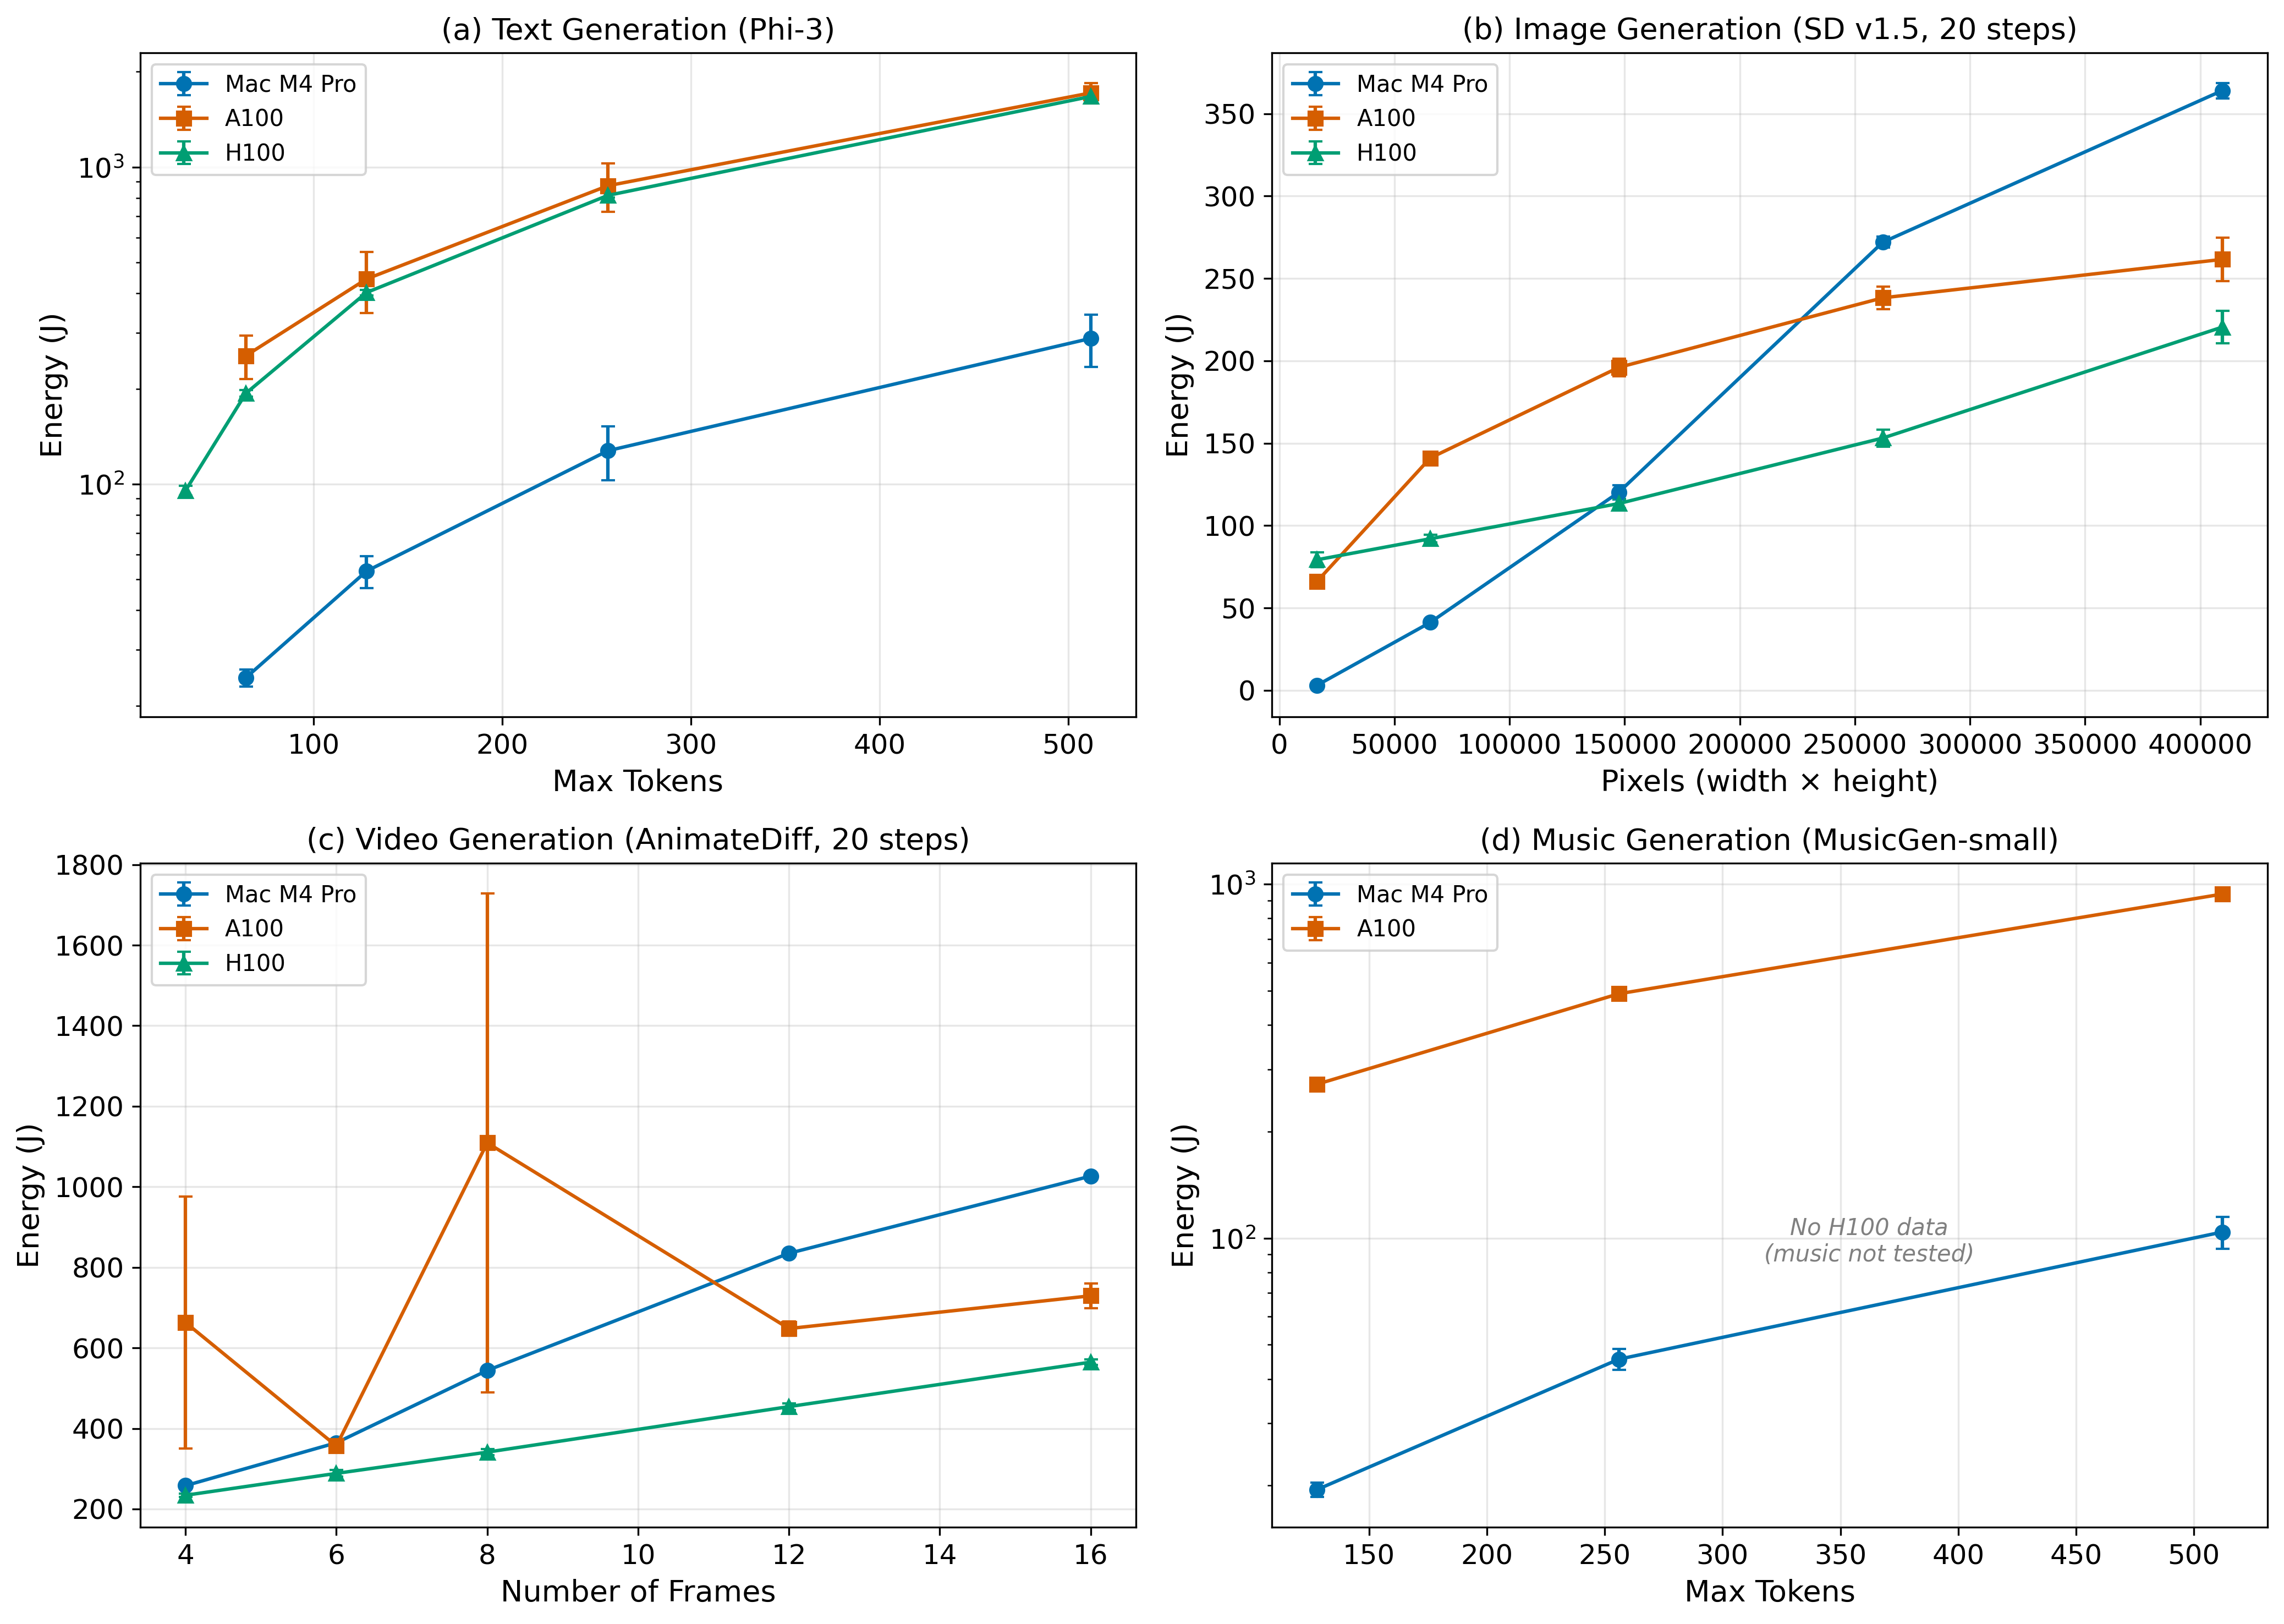
\includegraphics[width=0.95\textwidth]{../figures/fig1_3hw_comparison.png}
\caption{Energy consumption across four generative AI modalities on three hardware platforms. Comparison of Apple M4 Pro (blue), NVIDIA A100 (vermillion), and NVIDIA H100 (teal). Error bars: $\pm 1$ SD over 30 runs. Dashed lines: crossover points. The H100 shifts crossovers lower and eliminates the video crossover.}
\label{fig:4modal}
\end{figure}

\textbf{Text generation} (Phi-3, 3.8B). The Mac consumed 24.5\,J (64 tokens) to 288.2\,J (512 tokens), while the A100 consumed 254.2--1,715\,J ($6.0$--$10.4\times$ more) and the H100 consumed 193.4--1,671\,J ($5.8$--$7.9\times$ more). Despite 75\% higher TDP and $2.4\times$ more CUDA cores, the H100 saved only 3--24\% over the A100---the extra silicon does not help when the computation is sequential. All comparisons were statistically significant ($p < 10^{-20}$, Cohen's $d > 5$).

\textbf{Image generation} (SD v1.5, 0.9B). Here the crossover appears, and its location depends on the GPU. The Mac consumed 41.2\,J ($256^2$) to 272\,J ($512^2$) at 20 steps. On the A100, the crossover occurred between $384^2$ and $512^2$: at $256^2$ the A100 consumed $3.4\times$ more than the Mac, but at $512^2$ 12\% less. The H100 shifted this crossover lower: at $256^2$ it consumed $2.2\times$ more, but by $384^2$ it was 6\% cheaper, and at $512^2$ 44\% less.

\textbf{Video generation} (AnimateDiff). The A100 showed a crossover at ${\sim}7$ frames (note: A100 video data at 4 and 8 frames exhibited bimodal energy distributions due to cloud multi-tenancy; we use median values for these configurations---see Section~\ref{sec:limitations}). The H100, however, was cheaper at \emph{every} tested size: even for 4 frames it consumed 234\,J versus the Mac's 258\,J, and the gap widened to 46\% at 12 frames and 45\% at 16 frames. AnimateDiff's 3D UNet processes all frames in parallel, generating enough work to keep the H100 busy even at minimal frame counts.

\textbf{Music generation} (MusicGen, 589M--2.0B). This is the worst case for GPU deployment. The A100 consumed $9$--$14\times$ more energy than the Mac while running no faster (speedup $0.8$--$1.0\times$). The GPU's parallelism is entirely wasted on sequential token generation.

\subsection{Energy Scaling Laws: Strong Fits for Most Modalities, With Notable Exceptions}
\label{sec:scaling}

We modeled energy as a power law $E(N) = \alpha \cdot N^\beta$, where $N$ is the complexity parameter (tokens, pixels, or frames), inspired by the scaling-law framework of Kaplan et al.~\cite{kaplan2020scaling}. Table~\ref{tab:scaling} presents the fitted parameters.

\begin{table}[t]
\centering
\caption{Energy scaling law parameters ($E = \alpha \cdot N^\beta$). For diffusion workloads, the Mac exhibits superlinear scaling ($\beta > 1$) while GPUs show sublinear scaling ($\beta < 1$). Text and music scale near-linearly on all platforms. $^\dagger$H100 image fit has lower $R^2$ due to GPU startup overhead at low resolutions; see text.}
\label{tab:scaling}
\small
\begin{tabular}{@{}llcccc@{}}
\toprule
\textbf{Modality} & \textbf{Scaling var.} & \textbf{Platform} & $\boldsymbol{\alpha}$ & $\boldsymbol{\beta}$ & $\boldsymbol{R^2}$ \\
\midrule
\multirow{3}{*}{Text} & \multirow{3}{*}{Tokens} & Mac M4 Pro & 0.167 & 1.195 & 0.9999 \\
 & & A100 & 4.330 & 0.959 & 0.9995 \\
 & & H100 & 2.660 & 1.033 & 0.9999 \\
\midrule
\multirow{3}{*}{Image} & \multirow{3}{*}{Pixels} & Mac M4 Pro & $8 \times 10^{-6}$ & 1.395 & 0.9998 \\
 & & A100 & 2.249 & 0.374 & 0.9974 \\
 & & H100$^\dagger$ & 1.081 & 0.404 & 0.877 \\
\midrule
\multirow{3}{*}{Video} & \multirow{3}{*}{Frames} & Mac M4 Pro & 59.20 & 1.065 & 1.000 \\
 & & A100 & 155.19 & 0.570 & 0.989 \\
 & & H100 & 88.18 & 0.665 & 0.995 \\
\midrule
\multirow{2}{*}{Music} & \multirow{2}{*}{Tokens} & Mac M4 Pro & 0.058 & 1.200 & 1.000 \\
 & & A100 & 3.205 & 0.910 & 0.9995 \\
\bottomrule
\end{tabular}
\end{table}

\textbf{Strong scaling patterns ($R^2 > 0.99$).}\quad
For text, all three platforms produce excellent power-law fits ($R^2 \geq 0.9995$). The Mac and H100 show near-linear to slightly superlinear scaling ($\beta \approx 1.03$--$1.20$), while the A100 is slightly sublinear ($\beta = 0.96$). For video on all platforms and music on both tested platforms, fits are similarly strong. The exponent divergence is consistent: edge hardware scales superlinearly while GPUs scale sublinearly for diffusion workloads.

\textbf{Image generation on H100 ($R^2 = 0.877$).}\quad
The H100 image fit shows a notably lower $R^2$ compared to other modality--hardware combinations. This reflects two effects: (1)~GPU startup overhead is proportionally large at $128^2$ (79\,J, only $36\%$ of the $640^2$ value of 221\,J, despite a $25\times$ smaller workload), creating a ``floor'' that a simple power law cannot capture; and (2)~image complexity is inherently two-dimensional (resolution $\times$ steps), and a single-variable fit conflates these factors. When the $128^2$ point is excluded, the fit improves to $R^2 = 0.948$. The Mac and A100 image fits remain excellent ($R^2 > 0.997$) because their narrower resolution range (3 points at $256^2$--$512^2$) avoids the low-utilization regime.

\textbf{Key pattern.}\quad
The Mac exhibits superlinear scaling ($\beta > 1$) across all modalities, consistent with memory bandwidth saturation at higher complexity on the unified memory architecture. GPUs show sublinear scaling ($\beta < 1$) for diffusion workloads, reflecting improving utilization as larger workloads amortize idle power. For autoregressive workloads, all platforms scale near-linearly ($\beta \approx 0.96$--$1.20$), and the intercept difference ($\alpha_\text{GPU} / \alpha_\text{Mac} \approx 16$--$26\times$) precludes crossover within practical ranges.

\subsection{Crossover Points Depend on Architecture and GPU Generation}

The crossover point $N^*$---where a GPU achieves equal energy to edge---exists only when $\beta_\text{GPU} < \beta_\text{edge}$ and the intercept ratio permits crossing within practical ranges:
\begin{equation}
N^* = \left(\frac{\alpha_\text{edge}}{\alpha_\text{GPU}}\right)^{\frac{1}{\beta_\text{GPU} - \beta_\text{edge}}}
\end{equation}

GPU generation shifts these crossovers substantially (Figure~\ref{fig:ratio}):

\begin{itemize}[leftmargin=*]
\item \textbf{Image}: Mac--A100 crossover at ${\sim}217{,}000$ pixels ($\approx 466 \times 466$), confirmed empirically between $384^2$ and $512^2$. Mac--H100 crossover at ${\sim}142{,}000$ pixels ($\approx 377 \times 377$), confirmed between $256^2$ and $384^2$---a 35\% reduction.
\item \textbf{Video}: Mac--A100 crossover at ${\sim}7$ frames. For the H100, \textbf{no crossover}---it uses less energy at all tested sizes (4--16 frames, 9--46\% less).
\item \textbf{Text and music}: No crossover on either GPU. The Mac remains $5.8$--$10.4\times$ more efficient for text and $9$--$14\times$ for music.
\item \textbf{H100 vs.\ A100}: The H100 is $35$--$42\%$ more energy-efficient for image (at shared resolutions $256^2$--$512^2$) and $22$--$65\%$ for video, driven by $1.5$--$1.7\times$ faster completion despite $2.0$--$2.8\times$ higher power draw for image workloads (${\sim}1.4$--$2.0\times$ for video).
\end{itemize}

\begin{figure}[t]
\centering
\Description{Line charts showing GPU-to-Mac energy ratios for A100 and H100 across text, image, video, and music configurations, with the unity line marking the crossover.}
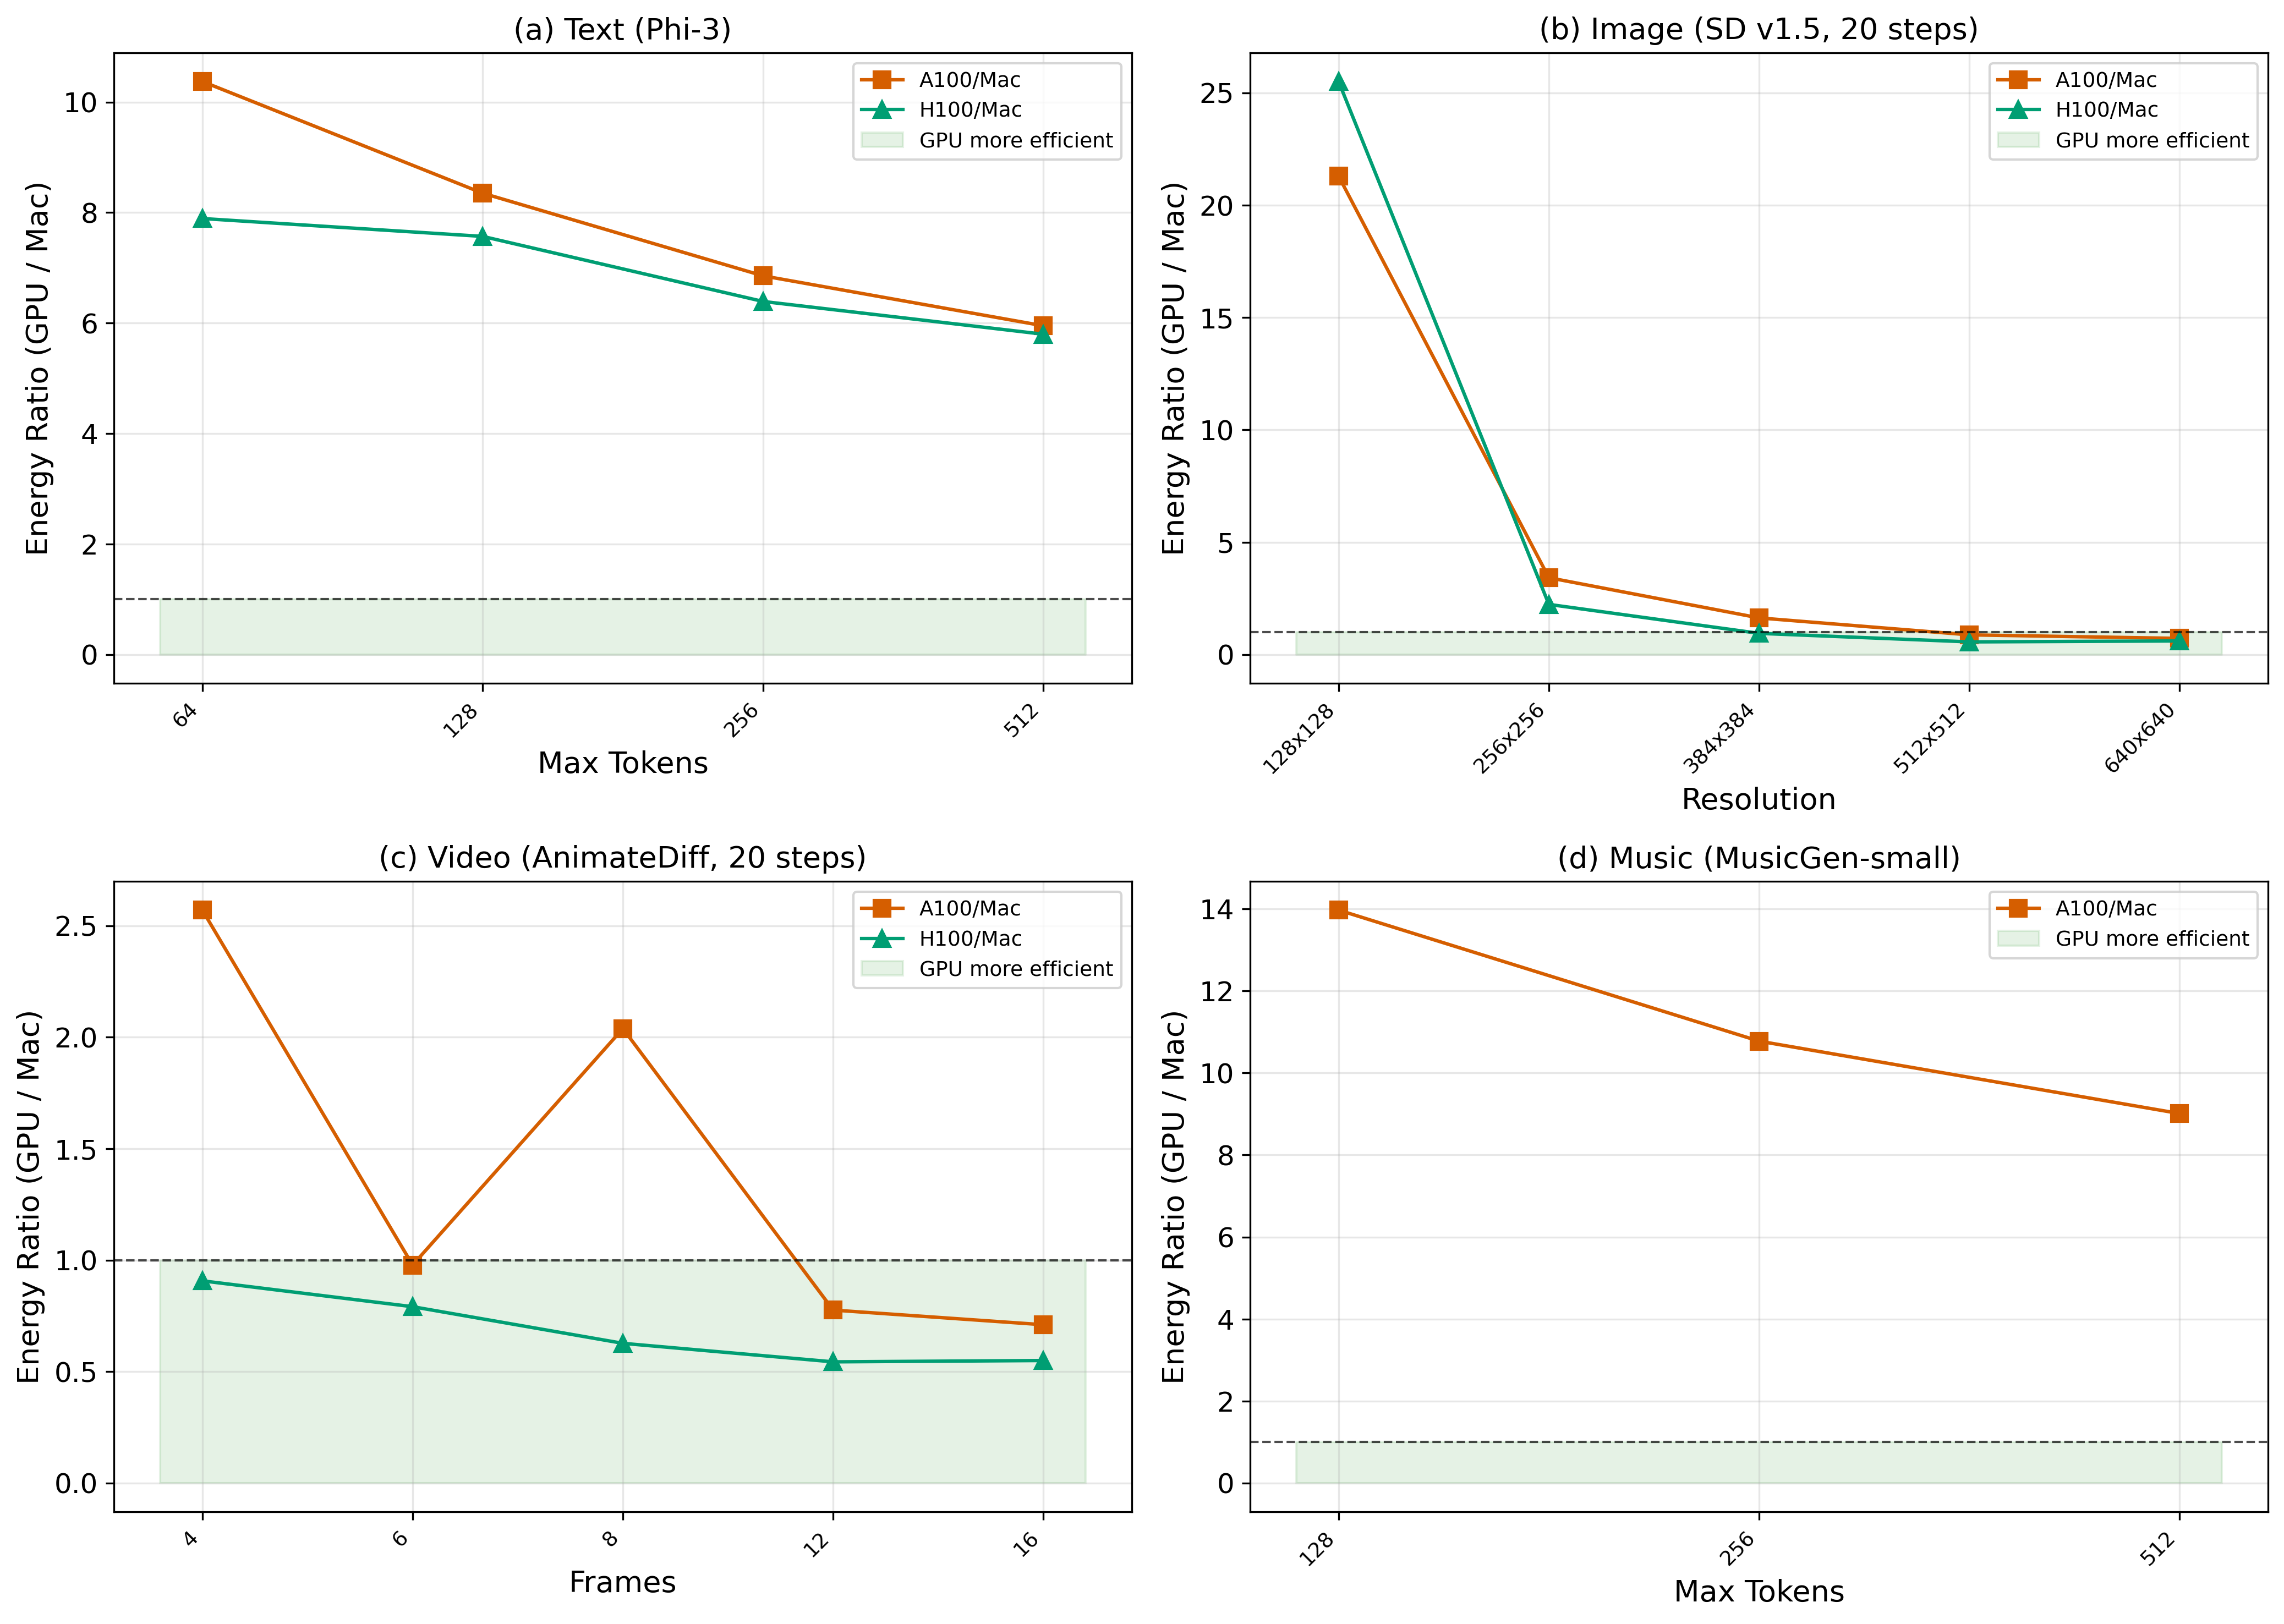
\includegraphics[width=0.95\textwidth]{../figures/fig2_efficiency_ratio_3hw.png}
\caption{Energy efficiency ratio across all configurations. Values below 1.0 indicate the GPU is more energy-efficient. The H100 crosses below 1.0 at lower complexity than the A100 for images, and remains below 1.0 for all video configurations.}
\label{fig:ratio}
\end{figure}

\subsection{The Speed--Energy Tradeoff: Four Operational Regimes}

Mapping each configuration in speed--energy space (Figure~\ref{fig:tradeoff}) reveals four regimes:

\begin{enumerate}[leftmargin=*]
\item \textbf{Worst case} (slower, more energy): Music on GPUs---no speed gain, $9$--$14\times$ energy penalty.
\item \textbf{Speed--energy tradeoff} (faster, more energy): Text and low-resolution image/video on A100.
\item \textbf{Best case} (faster, less energy): High-resolution image and multi-frame video on GPUs. The H100 achieves this for \emph{all} video and images $\geq 384^2$.
\item \textbf{GPU generational leap}: The H100 consistently shifts toward lower energy ratios vs.\ the A100.
\end{enumerate}

\begin{figure}[t]
\centering
\Description{Scatter plot showing speed ratio versus energy ratio for all configurations, with A100 as circles and H100 as squares, color-coded by modality.}
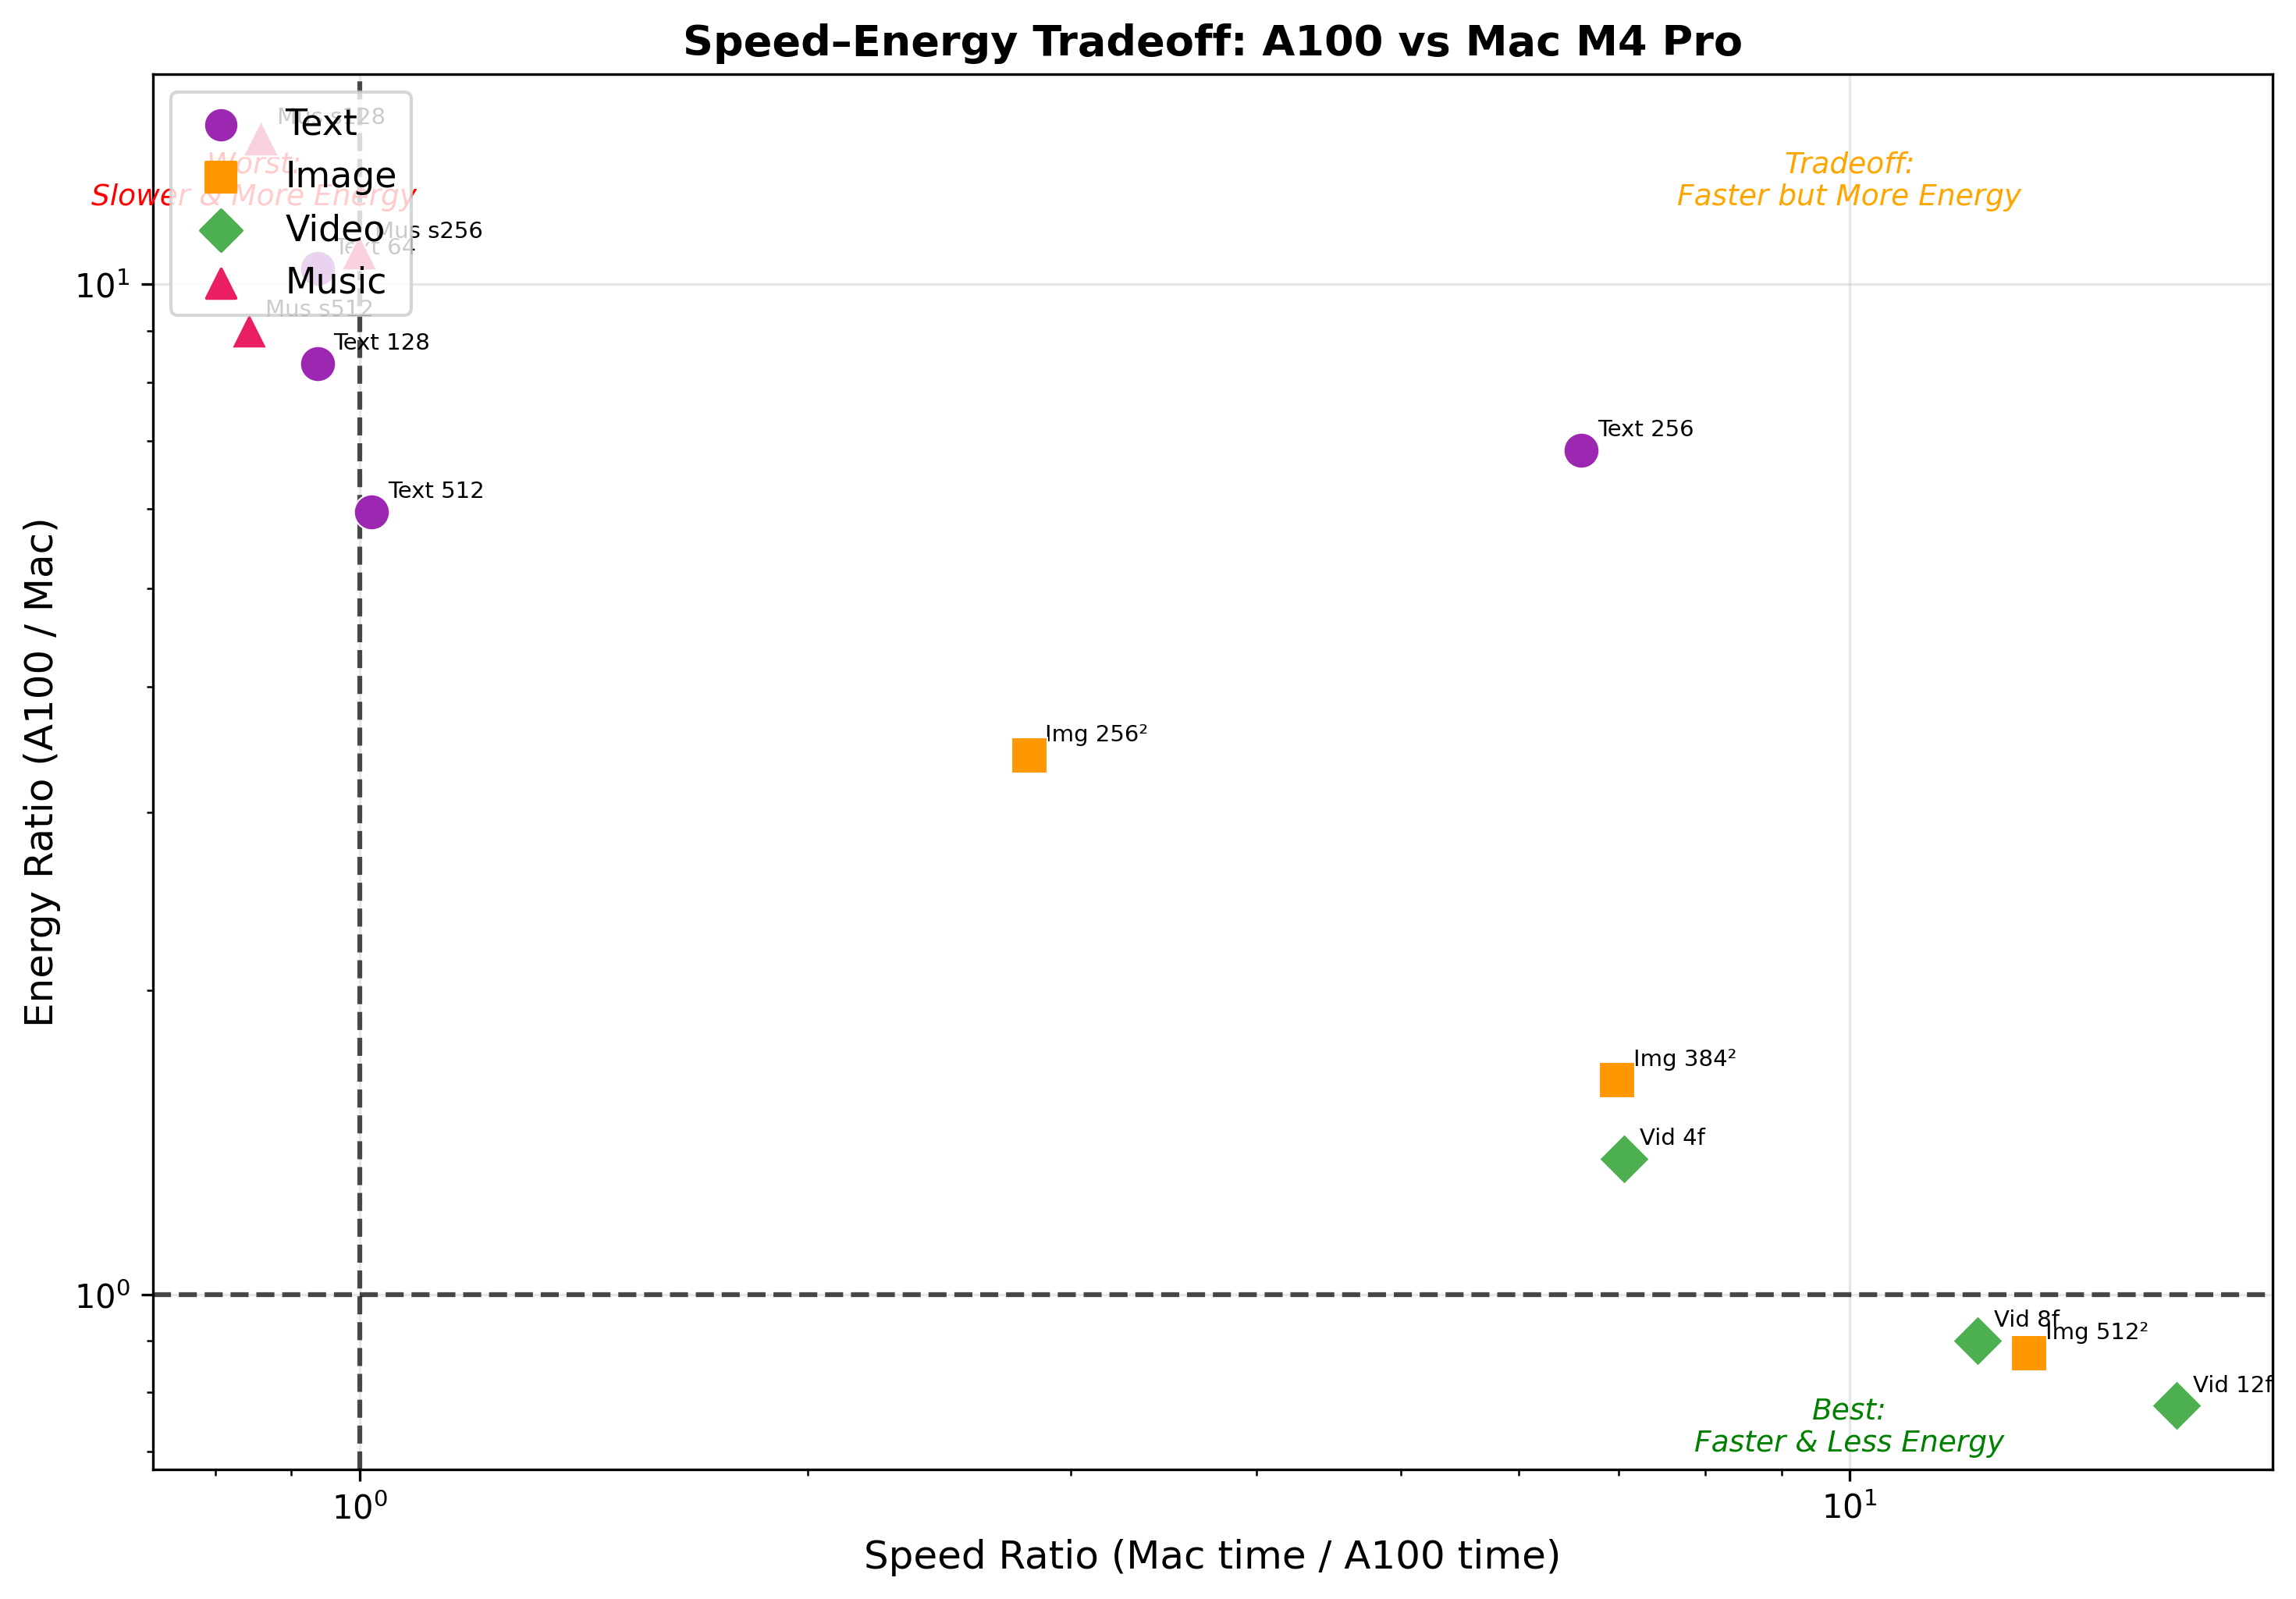
\includegraphics[width=0.85\textwidth]{../figures/fig5_speed_energy_tradeoff.png}
\caption{Speed--energy tradeoff. Each point is a modality--configuration pair. Points below $y=1$ and right of $x=1$ represent the best case (faster and cheaper on GPU).}
\label{fig:tradeoff}
\end{figure}

\subsection{Power Profiles Explain the Crossover Mechanism}

The A100 draws 63--279\,W, the H100 125--412\,W, and the Mac 6.4--24.3\,W. Since $E = P \cdot t$, the GPU achieves lower energy when its time reduction factor exceeds its power increase factor:

\begin{itemize}[leftmargin=*]
\item H100 Image $384^2$: speedup $14.9\times$ $>$ power ratio $14.5\times$ $\Rightarrow$ H100 wins (narrowly)
\item A100 Image $512^2$: speedup $6.7\times$ (by wall-clock duration) $>$ power ratio $5.9\times$ $\Rightarrow$ A100 wins
\item Music: speedup $0.9\times$ $<$ power ratio $7.7\times$ $\Rightarrow$ Mac wins by ${\sim}9$--$14\times$
\end{itemize}

The H100's power depends heavily on utilization: 160--190\,W at $128^2$ (23--27\% of TDP), rising to 378\,W average across all $640^2$ configurations (54\% of TDP; peak of 412\,W at $640^2$/50 steps). The Mac spans only ${\sim}4\times$ (6.4--24.3\,W). This explains why the crossover occurs only for diffusion workloads: only they generate sufficient parallel work to push GPU utilization above the energy-break-even threshold (Figure~\ref{fig:power}).

\begin{figure}[t]
\centering
\Description{Grouped bar chart showing average and peak power draw in watts for Mac, A100, and H100 across text, image, video, and music generation.}
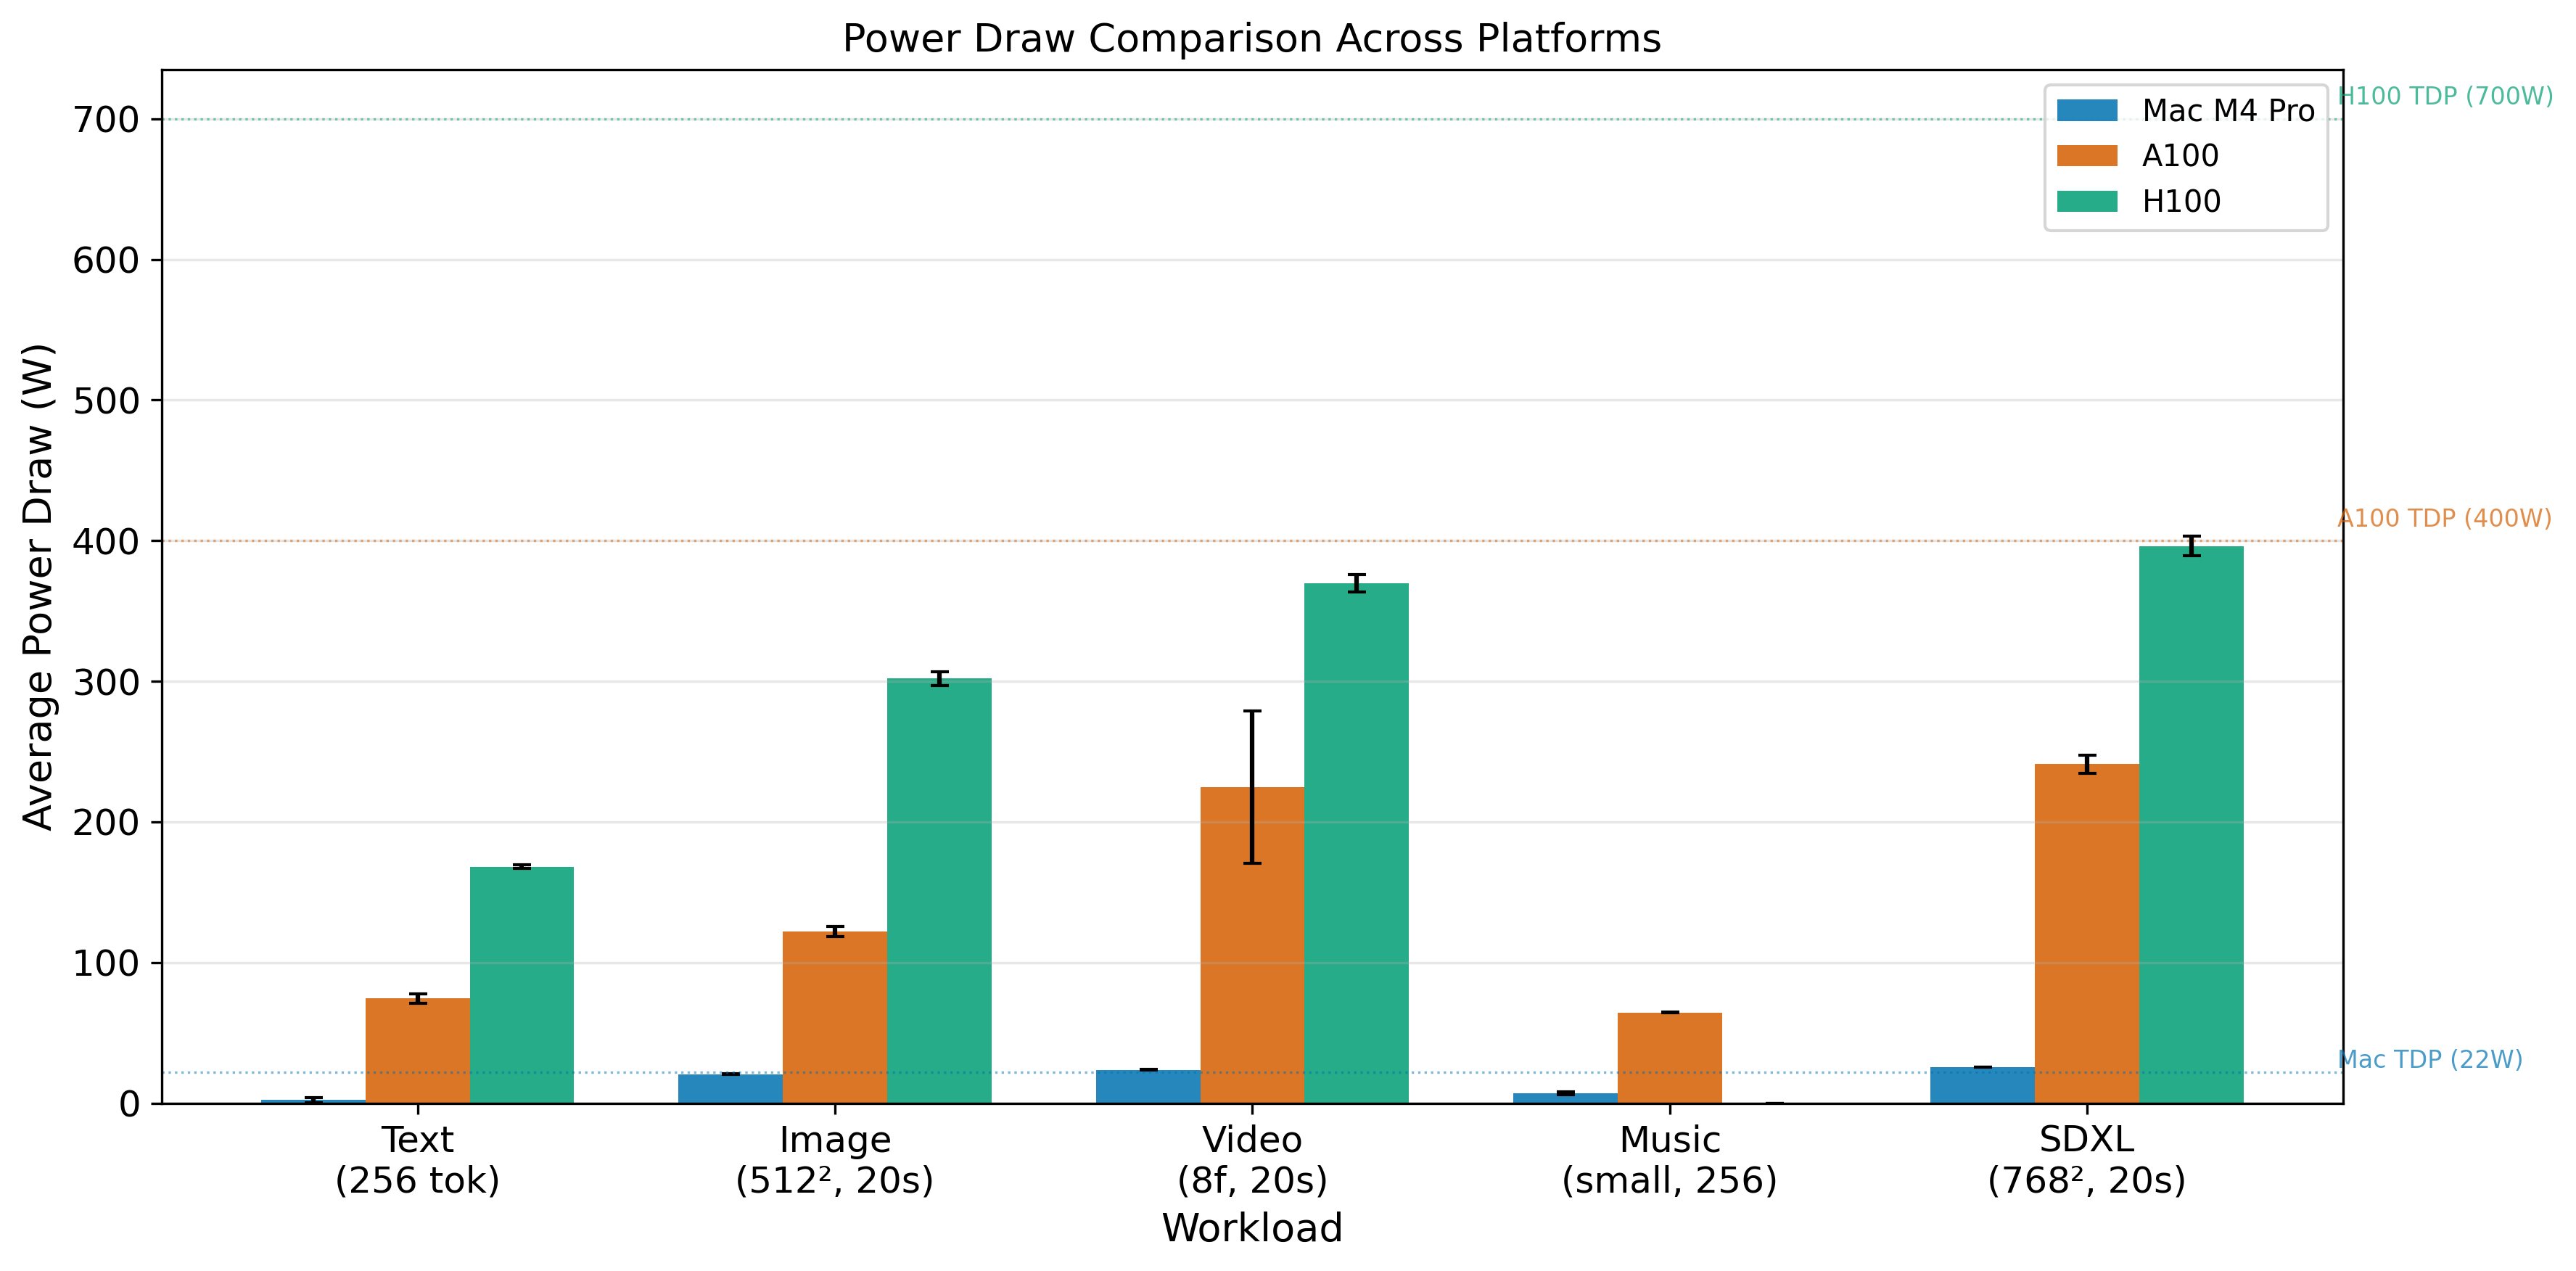
\includegraphics[width=0.95\textwidth]{../figures/fig8_power_profile_3hw.png}
\caption{Average and peak power draw across modalities. The H100 draws $2.0$--$2.8\times$ more power than the A100 for image workloads (${\sim}1.4$--$2.0\times$ for video) but achieves $1.5$--$1.7\times$ faster completion.}
\label{fig:power}
\end{figure}

\subsection{Cross-Model Validation: SDXL Confirms Patterns}

We repeated image experiments with SDXL-base-1.0~\cite{podell2023sdxl} (3.5B parameters, $3.9\times$ larger than SD~v1.5) across all three platforms. The crossover pattern persisted: the H100 consumed 35--40\% less energy than the A100, and achieved energy parity with the Mac at lower resolutions than for SD~v1.5, consistent with SDXL's higher computational intensity providing better GPU utilization. On the H100, SDXL at $1024^2$/30 steps consumed 945\,J with CLIP~0.33, while SD~v1.5 at $640^2$/50 steps consumed 537\,J with CLIP~0.29---demonstrating a hardware-dependent energy--quality tradeoff.

\subsection{Batched Inference: Narrows But Does Not Eliminate Edge Advantage}
\label{sec:batched}

Real-world GPU serving systems batch multiple queries. We measured batched Phi-3 inference on both GPUs with batch sizes 1--16. Per-query energy dropped dramatically: on the H100, from 889\,J (batch=1) to 69\,J (batch=16), a 92\% reduction; on the A100, from 876\,J to 115\,J, an 87\% reduction.

At batch=16, the H100's per-query energy (69\,J at 256 tokens) is \emph{lower} than the Mac's single-query energy at the same token count (127.5\,J at 256 tokens), demonstrating that aggressive batching can make GPU serving more energy-efficient than edge for text generation. However, this requires sustained high utilization: at batch=1, the H100 consumes $7.0\times$ more than the Mac (889\,J vs.\ 127.5\,J at 256 tokens), and batch sizes $\geq 8$ are needed to approach parity. For larger models (70B+) that exceed edge memory, GPU batching remains the only option, and the 92\% reduction at batch=16 underscores the importance of maximizing utilization.

\subsection{Energy--Quality Tradeoff}

We measured CLIP scores alongside energy for SD~v1.5 and SDXL across all three platforms. Three patterns emerged:
\begin{enumerate}[leftmargin=*]
\item Quality saturated well before maximum step counts: on the H100, SD~v1.5 reached CLIP $\approx 0.30$ at $512^2$ by 15 steps, while additional steps to 50 consumed $2.4\times$ more energy with no quality improvement.
\item Resolution had a larger effect on quality than step count: increasing from $256^2$ to $512^2$ improved CLIP by 0.08--0.10 points, while increasing steps from 20 to 50 at fixed resolution improved CLIP by only 0.01--0.02.
\item The energy--quality Pareto frontier is hardware-dependent. On the Mac, the most efficient path is moderate resolution with minimal steps ($384^2$/15 steps: CLIP~0.28, 16\,J). On the H100, higher resolution becomes competitive ($512^2$/15 steps: CLIP~0.30, 140\,J).
\end{enumerate}

These findings suggest that energy--quality-aware scheduling---routing to the optimal hardware \emph{and} truncating denoising at the saturation point---could reduce consumption by 50--60\% at negligible quality cost.

\subsection{Measurement Reliability}

Table~\ref{tab:reliability} shows coefficients of variation (CV) across 30 runs. Image and video measurements show excellent reproducibility ($<3.5\%$). Text CV is higher (17--19\%) due to variable output lengths from early EOS tokens. Music uses stochastic sampling, introducing additional variance.

\begin{table}[t]
\centering
\caption{Measurement reliability (CV across 30 runs).}
\label{tab:reliability}
\small
\begin{tabular}{@{}llccc@{}}
\toprule
\textbf{Modality} & \textbf{Configuration} & \textbf{Mac CV (\%)} & \textbf{A100 CV (\%)} & \textbf{H100 CV (\%)} \\
\midrule
Text & 256 tokens & 19.5 & 17.7 & 1.6 \\
Image & $512 \times 512$, 20 steps & 1.3 & 2.9 & 3.4 \\
Video & 8 frames, 20 steps & 0.6 & 2.7 & 2.2 \\
Music & Small, 256 tokens & 6.9 & 0.6 & -- \\
\bottomrule
\end{tabular}
\end{table}

%% ================================================================
\section{Discussion: Implications for AI Systems Deployment}
\label{sec:discussion}
%% ================================================================

\subsection{Modality-Aware Routing as a Systems Strategy}

The three-platform comparison points to a concrete systems opportunity: a \emph{modality-aware, hardware-aware routing strategy} that directs each query to the cheapest hardware for its workload type, with thresholds that depend on the available GPU generation.

For autoregressive workloads (text, music), routing to edge devices reduces per-query energy by $6$--$10\times$, regardless of whether the alternative is an A100 or H100. For diffusion workloads, the optimal routing depends on the available GPU: with H100-class hardware, all video and images $\geq 384^2$ should be GPU-routed for savings of 6--46\%. With A100-class hardware, only images $\geq 512^2$ and videos $\geq 8$ frames benefit.

Implementation is straightforward: an inference scheduler classifies each request by modality and complexity (resolution, frame count, or token length) and routes it to the energy-favorable platform. Our crossover thresholds provide the decision boundaries. No model modification is needed---the same checkpoint runs on both platforms.

\subsection{Cost and Latency Implications}

The energy crossover has direct cost implications. At current cloud GPU pricing (\$2--4/hr for A100, \$4--8/hr for H100), a text query costs ${\sim}0.001$--$0.003$ on a cloud GPU vs.\ ${\sim}0.0001$ on edge hardware (amortized). For diffusion workloads above the crossover, the GPU is both faster \emph{and} cheaper per query when utilization is high.

The latency dimension adds nuance. GPUs provide $10$--$20\times$ speedup for diffusion, which matters for user-facing applications. For text, the Mac is slightly slower (by $1.1$--$1.3\times$) but $6$--$10\times$ more energy-efficient, presenting a clear latency--energy tradeoff. In practice, the optimal deployment depends on whether the application is latency-sensitive (favor GPU for diffusion) or throughput/cost-sensitive (favor edge for autoregressive).

\subsection{Implications for Mixed-Fleet Operation}

Organizations operating mixed hardware fleets can apply these findings directly:

\begin{itemize}[leftmargin=*]
\item \textbf{H100 fleet}: Route all video, images $\geq 384^2$ to GPU; text and music to edge. Energy saving: 35--46\% for GPU-routed diffusion, $6$--$10\times$ for edge-routed autoregressive.
\item \textbf{A100 fleet}: Route images $\geq 512^2$ and videos $\geq 8$ frames to GPU; keep small diffusion workloads on edge. The routing threshold is higher, reducing GPU-side savings.
\item \textbf{Batching strategy}: When GPU utilization is high (batch $\geq 8$), per-query energy drops substantially. Scheduling systems should batch aggressively when edge routing is infeasible.
\end{itemize}

\subsection{The Architectural Divide: Why Crossover is Modality-Specific}

The crossover effect arises from a fundamental mismatch between computational paradigm and hardware design. Autoregressive models generate tokens sequentially, creating an inherently serial computation graph. The A100's 6,912 CUDA cores operate at high base power (63--80\,W even for small workloads) but cannot accelerate sequential generation proportionally. The Mac's unified memory architecture eliminates data transfer overhead and operates at 6--12\,W total, making it $9$--$14\times$ more efficient.

Diffusion models perform parallel denoising across spatial dimensions, creating workloads that can saturate GPU cores. At low resolutions, the workload is insufficient to justify the GPU's power overhead, but as resolution increases, GPU utilization improves: the A100 completes $512^2$ generation $6.7\times$ faster than the Mac (by wall-clock duration), and this speedup exceeds the $5.9\times$ power ratio.

This is reflected in the scaling fits: the Mac's $\beta > 1$ is consistent with memory bandwidth saturation, while GPUs' $\beta < 1$ for diffusion reflects improving utilization. The H100's text $\beta = 1.033$ (near-linear) reinforces the point: longer sequences do not create more parallelism for autoregressive decoding.

We note an alternative explanation: constant idle power captured by \texttt{powermetrics} (Mac) but excluded from \texttt{pynvml} (GPUs) could inflate the Mac's superlinearity. Our sensitivity analysis (Section~\ref{sec:sensitivity}) suggests this does not change qualitative conclusions.

\subsection{GPU Generational Trends}

Comparing A100 and H100 suggests a trend: each new GPU generation lowers the crossover for diffusion while leaving the autoregressive gap largely unchanged. The A100-to-H100 transition reduced the image crossover from ${\sim}466^2$ to ${\sim}377^2$ (35\%) and eliminated the video crossover entirely.

If this trend continues (B100/B200), we predict: image crossover drops below $256^2$, making GPUs energy-dominant across all practical resolutions; video remains GPU-dominant; but text generation stays edge-favored until GPU idle power drops below ${\sim}30$\,W or autoregressive decoding is replaced by a parallel alternative. The emergence of dedicated AI accelerators (Google TPU v5, AMD MI300X) may further diversify the landscape; our framework of measuring energy scaling exponents provides a general methodology applicable to any hardware pairing.

\subsection{Relation to Prior Work}

Luccioni et al.~\cite{luccioni2024power} found that image generation uses ${\sim}60\times$ more energy than text classification on an A100; we show this gap is hardware-dependent, with text becoming disproportionately cheaper on edge. GPU-only benchmarks~\cite{you2023zeus} may overestimate autoregressive inference costs by an order of magnitude relative to edge deployment. Samsi et al.~\cite{samsi2023words} found approximately linear energy-per-token scaling, consistent with our fits ($\beta \approx 0.96$--$1.20$). Iyengar et al.~\cite{castano2025energy} found FLOPs-based power-law scaling for diffusion on GPUs; we complement this by showing qualitatively different scaling on edge SoCs. Desislavov et al.~\cite{desislavov2023trends} noted efficiency gains follow hardware improvements; our modality-specific results show that hardware \emph{selection} can yield order-of-magnitude savings for appropriate workloads---orthogonal to generational improvements.

There is also a methodological point. Existing benchmarks~\cite{you2023zeus,jegham2025hungry,luccioni2024power} report values on fixed hardware, implicitly treating deployment as a constant. Our data show this can mislead: a model that looks energy-hungry on a GPU may be cheap on edge, and vice versa. Future benchmarks should cover at least two hardware tiers, and efficiency claims should state the deployment context.

%% ================================================================
\section{Sensitivity Analysis}
\label{sec:sensitivity}
%% ================================================================

GPU measurements via \texttt{pynvml} capture board power only, while Mac measurements via \texttt{powermetrics} include all subsystems. To test robustness, we applied a conservative 40\% overhead correction ($1.4\times$) to all GPU measurements, representing the upper bound of typical PUE values~\cite{wu2022sustainable}.

Even with this correction, autoregressive advantage remains $4.1$--$7.4\times$ (vs.\ $5.8$--$14\times$ uncorrected), the crossover persists, and all qualitative conclusions hold. The crossover point shifts to slightly lower resolutions but is not eliminated.

%% ================================================================
\section{Prompt Invariance Validation}
\label{sec:prompt}
%% ================================================================

To validate that energy is determined by computational configuration rather than prompt content, we tested 5 semantically distinct prompts per modality (text and image), each repeated 10 times on the Mac M4 Pro.

\textbf{Image generation} shows near-complete prompt invariance: across 5 diverse prompts at $512^2$/20 steps, the maximum difference between prompt means was only 2.0\% of the overall mean. The within-prompt variance was $6.7\times$ larger than between-prompt variance, confirming that configuration---not content---determines energy. \textbf{Text generation} shows slightly higher sensitivity (8.4\% range), driven by input tokenization differences, but within-prompt variance remained $12.1\times$ larger than between-prompt variance.

%% ================================================================
\section{Limitations}
\label{sec:limitations}
%% ================================================================

\begin{enumerate}[leftmargin=*]
\item \textbf{Measurement asymmetry}: GPU measurements exclude host CPU/system overhead; Mac measurements include all subsystems. For inference, GPU power dominates~\cite{patterson2021carbon,wu2022sustainable}, and our sensitivity analysis confirms robustness.

\item \textbf{Model size range}: All tested models are 589M--3.8B parameters. This scope is deliberate---the crossover question is meaningful only when both deployment options are viable---but limits applicability to larger models (70B+). For those, our batching results (Section~\ref{sec:batched}) provide relevant guidance. As edge memory grows (M4 Ultra: 192\,GB), the crossover analysis extends to larger models.

\item \textbf{Multi-tenant variability}: Colab-based GPU measurements may be affected by shared infrastructure. We observed bimodal energy distributions in A100 video experiments at 4 and 8 frames (e.g., clusters at ${\sim}335$\,J and ${\sim}1{,}015$\,J for 4 frames), likely due to shared cloud infrastructure variability. We report median values for these configurations to mitigate this effect and flag them as having higher measurement uncertainty. For all other configurations, our 30-repeat protocol yielded low CVs (0.6--3.4\% for image/video; Table~\ref{tab:reliability}).

\item \textbf{H100 image scaling law fit}: The single-variable power law achieves $R^2 = 0.877$ for H100 image generation (vs.\ $>0.99$ for other combinations), reflecting the two-dimensional nature of image complexity and GPU startup overhead. Multi-variable scaling models would improve this fit.

\item \textbf{Software versions}: PyTorch 2.4.1 on Mac vs.\ 2.1.0 on GPUs due to Colab constraints.

\item \textbf{Quality metrics}: We use CLIP scores for image quality. More comprehensive evaluation (FID, FVD, perplexity) would strengthen the energy--quality tradeoff analysis.

\item \textbf{Scope}: We do not test consumer GPUs (RTX 4090), mobile SoCs, or DiT-based image models. Network transfer energy is not accounted for.
\end{enumerate}

%% ================================================================
\section{Conclusion}
\label{sec:conclusion}
%% ================================================================

We presented a systematic cross-hardware, cross-modality energy benchmark revealing the Energy Crossover Effect: for diffusion workloads, energy-efficiency leadership shifts from edge to GPU as output complexity grows, while autoregressive workloads consistently favor edge hardware by $6$--$10\times$. The crossover threshold is GPU-generation-dependent and follows from the divergent scaling exponents of edge ($\beta > 1$) and GPU ($\beta < 1$) platforms.

For AI systems practitioners, the implication is clear: modality-aware routing---directing autoregressive workloads to edge hardware and sufficiently complex diffusion workloads to GPUs---can reduce energy consumption by up to an order of magnitude for text/music and 6--46\% for image/video, with no model modification required. As GPU hardware evolves, the crossover for diffusion will continue to shift toward smaller workloads, while the autoregressive gap will persist until GPU idle power drops dramatically or parallel decoding alternatives emerge.

%% ================================================================
\section*{AI Use Declaration}
%% ================================================================

The author used AI assistants for grammar checking and \LaTeX\ formatting. All experimental design, data collection, analysis, and interpretation were conducted by the author.

%% ================================================================
\section*{Data and Code Availability}
%% ================================================================

All experimental data (4,500+ JSON records across three hardware platforms), analysis scripts, and measurement notebooks are available at \url{https://github.com/yjkim0123/energy-crossover-effect}. All models used are publicly available via Hugging Face.

\begin{acks}
The A100 and H100 experiments were conducted on Google Colab Pro+. The author thanks NVIDIA for the open-source \texttt{pynvml} library and the developers of the open-weight models used in this study.
\end{acks}

\begin{thebibliography}{30}

\bibitem{iea2024}
International Energy Agency.
\newblock Energy and {AI}.
\newblock IEA, Paris, 2024.
\newblock \url{https://www.iea.org/reports/energy-and-ai}.

\bibitem{devries2023growing}
Alex de~Vries.
\newblock The growing energy footprint of artificial intelligence.
\newblock \emph{Joule}, 7(10):2191--2194, 2023.
\newblock \doi{10.1016/j.joule.2023.09.004}.

\bibitem{luccioni2024power}
Alexandra~Sasha Luccioni, Yacine Jernite, and Emma Strubell.
\newblock Power hungry processing: Watts driving the cost of {AI} deployment?
\newblock In \emph{Proc. ACM FAccT}, pages 85--99. ACM, 2024.
\newblock \doi{10.1145/3630106.3658542}.

\bibitem{strubell2019energy}
Emma Strubell, Ananya Ganesh, and Andrew McCallum.
\newblock Energy and policy considerations for deep learning in {NLP}.
\newblock In \emph{Proc. ACL}, pages 3645--3650, 2019.
\newblock \doi{10.18653/v1/P19-1355}.

\bibitem{patterson2021carbon}
David Patterson, Joseph Gonzalez, Quoc Le, Chen Liang, Lluis-Miquel Munguia, Daniel Rothchild, David So, Maud Texier, and Jeff Dean.
\newblock Carbon emissions and large neural network training.
\newblock \emph{arXiv preprint arXiv:2104.10350}, 2021.

\bibitem{luccioni2023bloom}
Alexandra~Sasha Luccioni, Sylvain Viguier, and Anne-Laure Ligozat.
\newblock Estimating the carbon footprint of {BLOOM}, a 176{B} parameter language model.
\newblock \emph{Journal of Machine Learning Research}, 24(253):1--15, 2023.

\bibitem{you2023zeus}
Jie You, Jae-Won Chung, and Mosharaf Chowdhury.
\newblock Zeus: Understanding and optimizing {GPU} energy consumption of {DNN} training.
\newblock In \emph{Proc. NSDI}, pages 119--139. USENIX, 2023.

\bibitem{samsi2023words}
Siddharth Samsi, Dan Zhao, Joseph McDonald, Baolin Li, Adam Michaleas, Michael Jones, William Bergeron, Jeremy Kepner, Devesh Tiwari, and Vijay Gadepally.
\newblock From words to watts: Benchmarking the energy costs of large language model inference.
\newblock In \emph{Proc. IEEE HPEC}, pages 1--9. IEEE, 2023.

\bibitem{dodge2022measuring}
Jesse Dodge, Taylor Prewitt, Remi~Tachet des Combes, Erika Odmark, Roy Schwartz, Emma Strubell, Alexandra~Sasha Luccioni, Noah~A. Smith, Nicole DeCario, and Will Buchanan.
\newblock Measuring the carbon intensity of {AI} in cloud instances.
\newblock In \emph{Proc. FAccT}, pages 1877--1894. ACM, 2022.
\newblock \doi{10.1145/3531146.3533234}.

\bibitem{wu2022sustainable}
Carole-Jean Wu, Ramya Raghavendra, Udit Gupta, Bilge Acun, Newsha Ardalani, Kiwan Maeng, Gloria Chang, Fiona Aga, Jinshi Huang, Charles Bai, Michael Gschwind, Anurag Gupta, Myle Ott, Anastasia Melnikov, Salvatore Candido, David Brooks, Geeta Chauhan, Benjamin Lee, Hsien-Hsin Lee, Bugra Akyildiz, Maximilian Balandat, Joe Spisak, Ravi Jain, Mike Rabbat, and Kim Hazelwood.
\newblock Sustainable {AI}: Environmental implications, challenges and opportunities.
\newblock In \emph{Proc. MLSys}, 2022.

\bibitem{desislavov2023trends}
Radosvet Desislavov, Fernando Mart{\'\i}nez-Plumed, and Jos{\'e} Hern{\'a}ndez-Orallo.
\newblock Trends in {AI} inference energy consumption: Beyond the performance-vs-parameter laws of deep learning.
\newblock \emph{Sustainable Computing: Informatics and Systems}, 38:100857, 2023.
\newblock \doi{10.1016/j.suscom.2023.100857}.

\bibitem{kaack2022aligning}
Lynn~H. Kaack, Priya~L. Donti, Emma Strubell, George Kamiya, Felix Creutzig, and David Rolnick.
\newblock Aligning artificial intelligence with climate change mitigation.
\newblock \emph{Nature Climate Change}, 12:518--527, 2022.
\newblock \doi{10.1038/s41558-022-01377-7}.

\bibitem{verdecchia2023systematic}
Roberto Verdecchia, June Sallou, and Lu{\'\i}s Cruz.
\newblock A systematic review of {Green AI}.
\newblock \emph{WIREs Data Mining and Knowledge Discovery}, 13:e1507, 2023.
\newblock \doi{10.1002/widm.1507}.

\bibitem{schwartz2020green}
Roy Schwartz, Jesse Dodge, Noah~A. Smith, and Oren Etzioni.
\newblock Green {AI}.
\newblock \emph{Communications of the ACM}, 63(12):54--63, 2020.
\newblock \doi{10.1145/3381831}.

\bibitem{abdin2024phi3}
Marah Abdin, Sam~Ade Jacobs, Ammar~Ahmad Awan, Jyoti Aneja, Ahmed Awadallah, Hany Awadalla, Nguyen Bach, Amit Bahree, Arash Bakhtiari, Harkirat Behl, et~al.
\newblock Phi-3 technical report: A highly capable language model locally on your phone.
\newblock \emph{arXiv preprint arXiv:2404.14219}, 2024.

\bibitem{rombach2022high}
Robin Rombach, Andreas Blattmann, Dominik Lorenz, Patrick Esser, and Bj{\"o}rn Ommer.
\newblock High-resolution image synthesis with latent diffusion models.
\newblock In \emph{Proc. CVPR}, pages 10684--10695. IEEE, 2022.
\newblock \doi{10.1109/CVPR52688.2022.01042}.

\bibitem{guo2024animatediff}
Yuwei Guo, Ceyuan Yang, Anyi Rao, Zhengyang Liang, Yaohui Wang, Yu Qiao, Maneesh Agrawala, Dahua Lin, and Bo Dai.
\newblock {AnimateDiff}: Animate your personalized text-to-image diffusion models without specific tuning.
\newblock In \emph{Proc. ICLR}, 2024.

\bibitem{copet2024musicgen}
Jade Copet, Felix Kreuk, Itai Gat, Tal Remez, David Kant, Gabriel Synnaeve, Yossi Adi, and Alexandre D{\'e}fossez.
\newblock Simple and controllable music generation.
\newblock In \emph{Proc. NeurIPS}, volume~36, 2023.

\bibitem{kaplan2020scaling}
Jared Kaplan, Sam McCandlish, Tom Henighan, Tom~B. Brown, Benjamin Chess, Rewon Child, Scott Gray, Alec Radford, Jeffrey Wu, and Dario Amodei.
\newblock Scaling laws for neural language models.
\newblock \emph{arXiv preprint arXiv:2001.08361}, 2020.

\bibitem{mao2024green}
Yuyi Mao, Xianghao Yu, Kaibin Huang, Ying-Jun~Angela Zhang, and Jun Zhang.
\newblock Green edge {AI}: A contemporary survey.
\newblock \emph{Proceedings of the IEEE}, 112(7):880--911, 2024.
\newblock \doi{10.1109/JPROC.2024.3437365}.

\bibitem{jegham2025hungry}
Nada Jegham, Marwane Abdelatti, Loubna Elmoubarki, and Abdeltawab Hendawi.
\newblock How hungry is {AI}? {Benchmarking} energy, water, and carbon footprint of {LLM} inference.
\newblock \emph{arXiv preprint arXiv:2505.09598}, 2025.

\bibitem{castano2025energy}
Aniruddha Iyengar, Jiaqi Han, Boris Ruf, Vincent Grari, Marcin Detyniecki, and Stefano Ermon.
\newblock Energy scaling laws for diffusion models: Quantifying compute and carbon emissions in image generation.
\newblock \emph{arXiv preprint arXiv:2511.17031}, 2025.

\bibitem{xu2024edge}
Xubin Wang et~al.
\newblock Cognitive edge computing: A comprehensive survey on optimizing large models and {AI} agents for pervasive deployment.
\newblock \emph{arXiv preprint arXiv:2501.03265}, 2025.

\bibitem{henderson2020towards}
Peter Henderson, Jieru Hu, Joshua Romoff, Emma Brunskill, Dan Jurafsky, and Joelle Pineau.
\newblock Towards the systematic reporting of the energy and carbon footprints of machine learning.
\newblock \emph{Journal of Machine Learning Research}, 21(248):1--43, 2020.

\bibitem{lacoste2019quantifying}
Alexandre Lacoste, Alexandra Luccioni, Victor Schmidt, and Thomas Dandres.
\newblock Quantifying the carbon emissions of machine learning.
\newblock \emph{arXiv preprint arXiv:1910.09700}, 2019.

\bibitem{anthony2020carbontracker}
Lasse~F.~Wolff Anthony, Benjamin Kanding, and Raghavendra Selvan.
\newblock Carbontracker: Tracking and predicting the carbon footprint of training deep learning models.
\newblock In \emph{ICML Workshop on Challenges in Deploying and Monitoring ML Systems}, 2020.

\bibitem{ho2020denoising}
Jonathan Ho, Ajay Jain, and Pieter Abbeel.
\newblock Denoising diffusion probabilistic models.
\newblock In \emph{Proc. NeurIPS}, volume~33, pages 6840--6851, 2020.

\bibitem{vaswani2017attention}
Ashish Vaswani, Noam Shazeer, Niki Parmar, Jakob Uszkoreit, Llion Jones, Aidan~N. Gomez, {\L}ukasz Kaiser, and Illia Polosukhin.
\newblock Attention is all you need.
\newblock In \emph{Proc. NeurIPS}, volume~30, 2017.

\bibitem{podell2023sdxl}
Dustin Podell, Zion English, Kyle Lacey, Andreas Blattmann, Tim Dockhorn, Jonas M{\"u}ller, Joe Penna, and Robin Rombach.
\newblock {SDXL}: Improving latent diffusion models for high-resolution image synthesis.
\newblock In \emph{Proc. ICLR}, 2024.

\bibitem{garcia2019estimation}
Eva Garc{\'\i}a-Mart{\'\i}n, Crefeda~Faviola Rodrigues, Graham Riley, and H{\aa}kan Grahn.
\newblock Estimation of energy consumption in machine learning.
\newblock \emph{Journal of Parallel and Distributed Computing}, 134:75--88, 2019.
\newblock \doi{10.1016/j.jpdc.2019.07.007}.

\end{thebibliography}

\end{document}
